\documentclass[10pt,twocolumn,letterpaper]{article}

\usepackage{cvpr}
\usepackage{times}
\usepackage{epsfig}
\usepackage{graphicx}
\graphicspath{{images/}}
\usepackage{amsmath}
\usepackage{amssymb}

\usepackage{subcaption}

% Include other packages here, before hyperref.

% If you comment hyperref and then uncomment it, you should delete
% egpaper.aux before re-running latex.  (Or just hit 'q' on the first latex
% run, let it finish, and you should be clear).
\usepackage[pagebackref=true,breaklinks=true,letterpaper=true,colorlinks,bookmarks=false]{hyperref}

\cvprfinalcopy % *** Uncomment this line for the final submission

\def\cvprPaperID{****} % *** Enter the CVPR Paper ID here
\def\httilde{\mbox{\tt\raisebox{-.5ex}{\symbol{126}}}}

% Pages are numbered in submission mode, and unnumbered in camera-ready
\ifcvprfinal\pagestyle{empty}\fi
\begin{document}

%%%%%%%%% TITLE
\title{Something Using Something}

\author{Ankan Bansal\\
%UMD\\
%Institution1 address\\
%{\tt\small firstauthor@i1.org}
% For a paper whose authors are all at the same institution,
% omit the following lines up until the closing ``}''.
% Additional authors and addresses can be added with ``\and'',
% just like the second author.
% To save space, use either the email address or home page, not both
\and
Joaquin Zepeda\\
%Amazon\\
%First line of institution2 address\\
%{\tt\small secondauthor@i2.org}
}

\maketitle
%\thispagestyle{empty}


%%%%%%%%% ABSTRACT
\begin{abstract}
	We present an approach based on clustering penalties for semi-supervised image classification.
	The proposed penalties can incorporate prior knowledge about the data distribution in the
	learning pipeline. The first penalty (called Mean Entropy Loss (MEL)) encourages the classifier
	to be more confident of the predictions, while the second (called Negative Batch Entropy Loss
	(NBEL)) enforces prior knowledge about the distribution of classes in the training dataset. We
	evaluate our approach in the semi-supervised setting on ImageNet and CIFAR-10 datasets. 
\end{abstract}


\section{Introduction}

\subsection{Motivation}
\begin{frame}
	\frametitle{Introduction}
	\begin{itemize}
		\item Collecting images is easy\\
			
\includegraphics[scale=0.2, center]{images/google}
		\item Getting annotations for them is hard\\
			
\includegraphics[scale=0.2, center]{images/amt}
		\item Need for algorithms that can utilize the unlabeled data
			\begin{itemize}
				\item Unsupervised - Representation Learning
				\item Weakly-supervised - Learning from coarse annotations
				\item Semi-supervised - Using both labeled and unlabeled data
			\end{itemize}
	\end{itemize}
\end{frame}

\subsection{Semi-Supervised Learning}
%\begin{frame}
%	\frametitle{Semi-Supervised Learning}
%	\begin{itemize}
%		\item Some labeled data available and the rest unlabeled
%		\item Use both to build better models
%	\end{itemize}
%\end{frame}

\begin{frame}
	\frametitle{Semi-Supervised Image Classification}
	\begin{itemize}
		\item Given two sets of images:
			\begin{itemize}
				\setlength\itemsep{0.5em}
				\item Labeled: $\mathcal{S} = \{(\mathbf{X}_i, y_i)\}_{i=1}^S$\\
				\item Unlabeled: $\mathcal{U} = \{\mathbf{X}_j\}_{j=S+1}^{S+U}$
			\end{itemize}
		\item Train an image classifier, $f(\mathbf{X};\Theta)$, which
			outputs a probability distribution, $\mathbf{q} = f(\mathbf{X}; \Theta)$, over classes $\mathcal{C}$
	\end{itemize}
\end{frame}

\subsection{Overview}
\begin{frame}
	\frametitle{Overview}
	\begin{itemize}
		\item We present unsupervised clustering and locality penalties
		\item Clustering encode knowledge about dataset class distribution
		\item Locality encodes the idea that objects occupy small regions
		\item No modifications to existing CNN architectures
		\item These can be used with cross-entropy for end-to-end training
	\end{itemize}
\end{frame}

\section{Approach}
\begin{frame}
	\frametitle{Approach}
	\begin{itemize}
		\item We introduce three unsupervised losses which can be used with supervised losses during
			training
		\item The first two can be considered clustering losses
			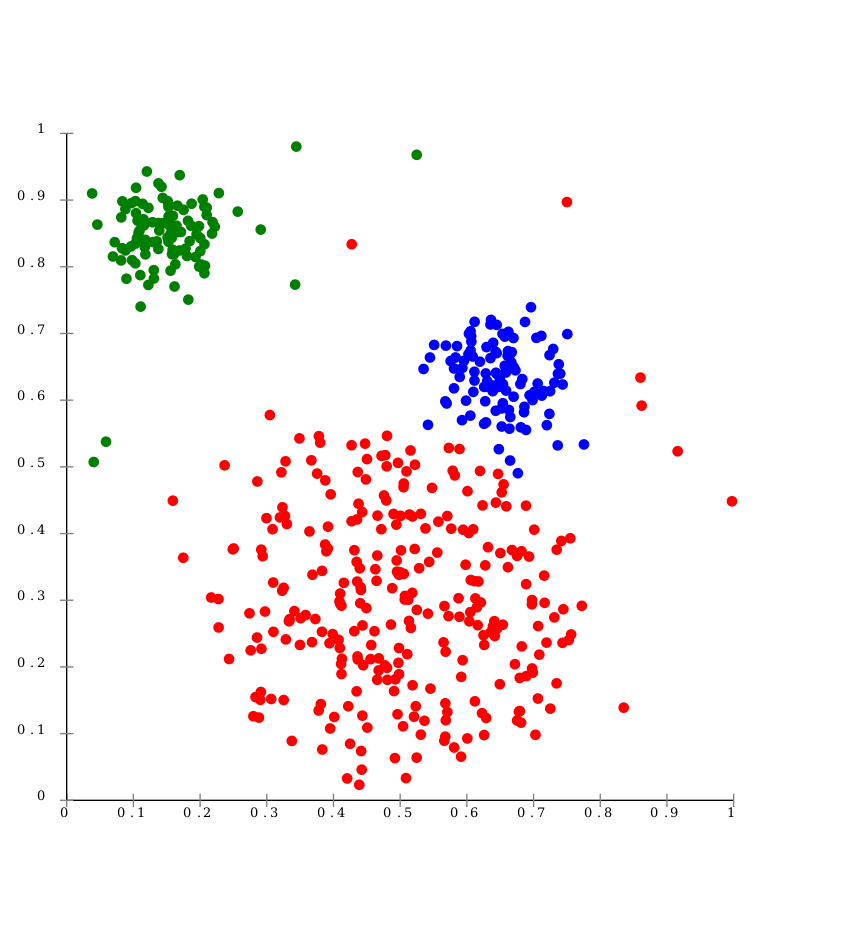
\includegraphics[width=0.4\textwidth, height=0.2\textwidth, center]{images/clust2}
		\item The third is a locality penalty
			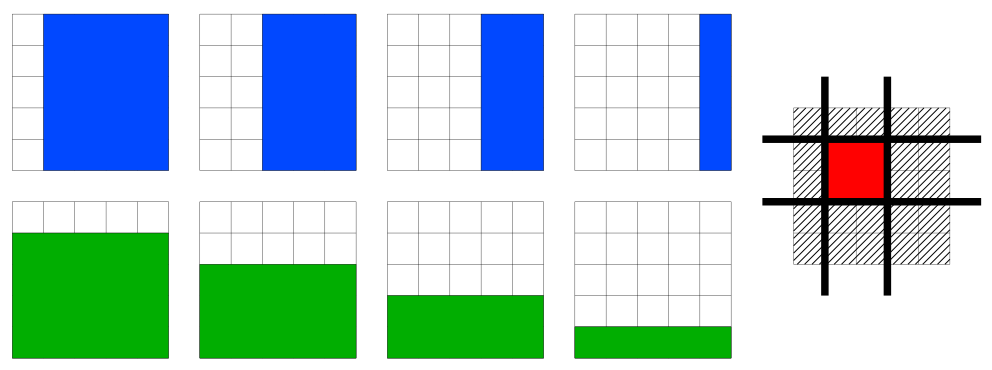
\includegraphics[scale=0.3, center]{images/locality}
	\end{itemize}
\end{frame}

\subsection{Clustering Losses}

\begin{frame}
	\frametitle{Clustering Losses}
	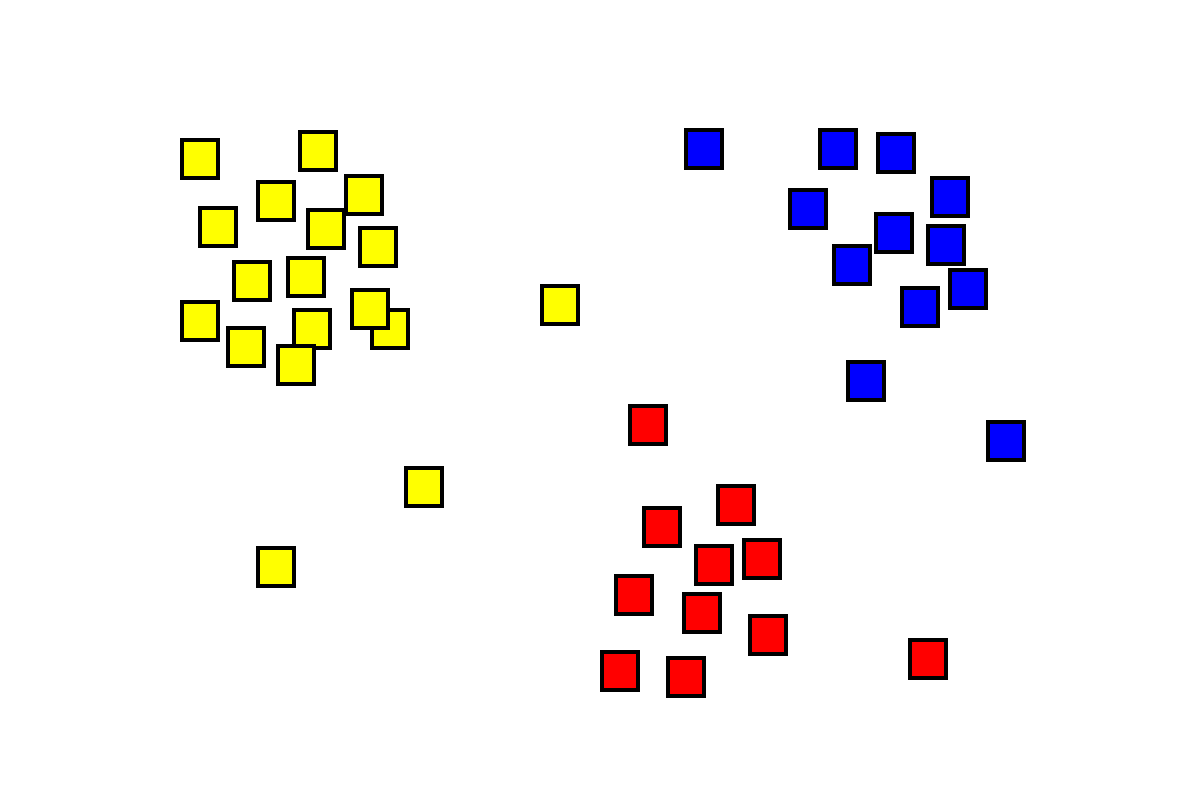
\includegraphics[scale=0.2, center]{images/clust1}
\end{frame}

\begin{frame}
	\frametitle{Mean Entropy Loss}
	\begin{itemize}
		\item The mean entropy loss over a batch of size $T$ is gives by:
			\begin{block}{Mean Entropy Loss (MEL)}
				\begin{equation*}
					J_M = \frac{1}{T}\sum_{t=1}^{T}H(\mathbf{q}_t)
				\end{equation*}
				where $H$ is the entropy and $\mathbf{q}_t = f(\mathbf{X}_t; \Theta)$ is the output
				probability distribution for image $\mathbf{X}_t$
			\end{block}
			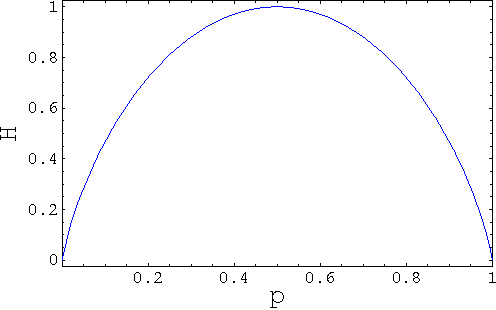
\includegraphics[scale=0.18, center]{images/ent.png}
		\item This increases the confidence of the predicted class
	\end{itemize}
\end{frame}

\begin{frame}
	\frametitle{Negative Batch Entropy Loss}
	\begin{itemize}
		\item The spread of outputs should be similar to the dataset
			label distribution
			\begin{block}{NBEL for Uniform Dataset Label Distribution}
				\begin{equation*}
					J_B = -H(\bar{\mathbf{q}})
				\end{equation*}
				where,
				\begin{equation*}
					\bar{\mathbf{q}} = \frac{1}{T}\sum_{t=1}^{T}\mathbf{q}_t
				\end{equation*}
			\end{block}

	\end{itemize}
\end{frame}

\begin{frame}
	\frametitle{Negative Batch Entropy Loss}
	\begin{itemize}
		\item Can be generalized to any distribution
			\begin{block}{Negative Batch Entropy Loss}
				\begin{equation*}
					\label{eq:nbel}
					J_B = D_{KL} (\bar{\mathbf{q}} \lVert \mathbf{d})
				\end{equation*}
				where $D_{KL}$ is the KL-divergence, and $\mathbf{d}$ is
				the empirical class distribution estimated from $\mathcal{S}$
			\end{block}

	\end{itemize}
\end{frame}


\subsection{Cross Entropy and Clustering}
\begin{frame}
	\frametitle{Adding Cross Entropy Loss}
	\begin{itemize}
		\item For a mini-batch, $\mathcal{B} = \{(\mathbf{X}_k, y_k)\}_{k=1}^R \cup
			\{\mathbf{X}_k\}_{k=R+1}^T$, where $\{(\mathbf{X}_k, y_k)\}_{k=1}^{R} \subseteq
			\mathcal{S}$, and $\{\mathbf{X}_k\}_{k=R+1}^{T} \subseteq \mathcal{U}$, the total loss
			can be give as:
			\begin{block}{Cross Entropy + Clustering}
				\begin{equation*}
					\mathcal{L} = J_C + \alpha J_M + \beta J_B
				\end{equation*}
				\begin{equation*}
					\mathcal{L} = \frac{1}{R} \sum_{t=1}^{R} E_t + \alpha \frac{1}{T}\sum_{t=1}^{T}H(\mathbf{q}_t) +
					\beta D_{KL}(\frac{1}{T}\sum_{t=1}^{T}\mathbf{q}_t \lVert \mathbf{d})
				\end{equation*}
			\end{block}
	\end{itemize}
\end{frame}


%\subsection{Sampling Ratio}
\begin{frame}
	\frametitle{Sampling Ratio}
	\begin{itemize}
		\item Each batch contains both labeled and unlabeled images
		\item Learning depends on their relative importance ($\frac{R}{T}$)
		%\item A higher $\frac{R}{T}$ means that supervised data and losses are considered more
		%	important
	\end{itemize}
\end{frame}


\subsection{Locality Loss}

\begin{frame}
	\frametitle{Locality Loss}
	\begin{itemize}
		\item Consider a class activation map (CAM) \footnote{\tiny{B. Zhou, A. Khosla, A.
				Lapedriza, A. Oliva, and A. Torralba. Learning Deep Features for Discriminative
		Localization.}}, $C \in \mathbb{R}^{N \times N}$. Let $\mathcal{G} = \{g_i
			\subseteq \textrm{support}(C)\}_i$ where $\textrm{support}(C) = [1 \dots N] \times [1
			\dots N]$ and $\cup_{g \in \mathcal{G}} = \textrm{support}(C)$
		\item The following norm induces group sparsity:
	\end{itemize}

	\begin{block}{Sparsity Norm}
		\begin{equation*}
			\Omega (C, \mathcal{G}) = \sum_{g \in \mathcal{G}} \left\lVert C_g \right\rVert _2
		\end{equation*}
		where $C_g$ is the vector formed by the values in $C$ indexed by $g$ and $\left\lVert . \right\rVert_2$ is
		the $L$-$2$ norm.
	\end{block}
\end{frame}


\begin{frame}
	\frametitle{Locality Loss}

	\begin{itemize}
		\item We use four sets $\mathcal G_i = \{g_{ik}\}_{k=1}^N$ corresponding, respectively, to nested
	left-to-right and right-to-left columns, and nested top-to-bottom and bottom-to-top columns,
	\textit{i.e.,}
	\end{itemize}
	\begin{block}{Groups}
		\vspace{-15pt}
		\begin{align*}
			g_{1k} & = [1 \ldots N] \times [1 \ldots k] \\
			g_{2k} & = [1 \ldots N] \times [N-k+1 \ldots N] \\
			g_{3k} & = [1 \ldots k] \times [1 \ldots N] \\
			g_{4k} & = [N-k+1 \ldots N] \times [1 \ldots N]
		\end{align*}
	\end{block}

	\vspace{-10pt}
	\begin{figure}
		\subfigure{
\includegraphics[scale=0.25]{images/g1}}~~
		\subfigure{
\includegraphics[scale=0.25]{images/g2}}~~
		\subfigure{
\includegraphics[scale=0.25]{images/g3}}
	\end{figure}
\end{frame}


\begin{frame}
	\frametitle{Locality Loss}
	\begin{itemize}
		\item The locality-inducing penalty for class $i$ for an image $\mathbf{X}_t$ is:
			\begin{block}{}
				\begin{equation*}
					J_{L,t}^{i} = \sum_{j=1}^{4}\Omega(C^i_t, \mathcal G_j)
				\end{equation*}
				where $C^i_{t}$ is the CAM for class $i$
			\end{block}
		\item Given $\mathbf{q}_t = f(\mathbf{X}_t; \Theta)$, we define our locality-inducing penalty to be
			\begin{block}{}
				\begin{equation*}
					J_{L,t} = \sum_{i} q_{ti} J_{L,t}^i
				\end{equation*}
			\end{block}
		\item The total locality penalty for a batch is $J_L =  \frac{1}{T} \sum_{t=1}^T J_L^t$
	\end{itemize}
\end{frame}

\subsection{Total Loss}
\begin{frame}
	\frametitle{Total Loss}
	\begin{itemize}
		\item Supervised losses (cross-entropy) applied only on labeled data
		\item Unsupervised losses can be applied on both
		\item Our total loss is given as:
	\end{itemize}
	\begin{block}{Total Loss}
		\begin{equation*}
			\mathcal{L} = J_C + \alpha J_M + \beta J_B + \gamma J_L
		\end{equation*}
		where $J_C$ is the cross-entropy loss, $J_M$ is mean entropy loss, $J_B$ is negative batch
		entropy loss, and $J_L$ is the locality loss
	\end{block}
\end{frame}


\section{Experiments}
\begin{frame}
	\frametitle{Experiments}
	\framesubtitle{Test Frame}
	Test
	\begin{itemize}
		\item Test
	\end{itemize}
	\begin{block}{Test}
		Test
	\end{block}
\end{frame}


\section{Related Work}

% Just putting some points and references here. 
\begin{itemize}
	\item Omni-supervised Learning - \cite{Radosavovic2017}
	\begin{itemize}
		\item Special regime of semi-supervised learning
		\item Ensemble the predictions from multi-transform inference in  a way that generates ``hard"
			labels
		\item Use more data from the internet as the unsupervised data
	\end{itemize}

	\item Mutual Exclusivity - \cite{Sajjadi2016}
	\begin{itemize}
		\item They us an unsupervised regularization term that explicitly forces the classifier's
			prediction for multiple classes to be mutually exclusive 
		\item This is the same condition as MEL 
	\end{itemize}
	
	\item Entropy Minimization - \cite{Grandvalet2005}
	\begin{itemize}
		\item Exactly MEL
		\item But applied on a very small scale. No experiments with large data
	\end{itemize}
	
	\item CatGAN - \cite{Springenberg2015}
	\begin{itemize}
		\item See notes/paper for this. This has lots of important material.  
		\item Uses MEL and NBEL as regularizers
	\end{itemize}
	
	\item Ladder Net - \cite{Rasmus2015}
	\begin{itemize}
		\item Read
	\end{itemize}
	
	\item Improved Techniques for Training GANs - \cite{Salimans2016}
	\begin{itemize}
		\item The discriminator of a GAN can be used to classify the images into $K+1$ categories
			instead of just two (real vs fake). These $K+1$ categories include the $K$ classes and the
			extra category for generated data
	\end{itemize}
	
	\item Temporal Ensembling - \cite{Laine2016}
	\begin{itemize}
		\item Self-ensembling where a consensus prediction is formed for the unknown labels using the
			outputs of the network-in-training on different epochs
		\item Used an unsupervised loss weighting function which ramps up with time starting from zero
	\end{itemize}
	
	\item Virtual Adversarial Training - \cite{Miyato2017}
	\begin{itemize}
		\item Local Distributional Smoothness (LDS) - The distribution of classification should be
			smooth around data points
		\item The goal is to improve the smoothness of the model in the neighborhood of all the observed
			inputs
	\end{itemize}
	
	\item Regularization with Stochastic Transformations - \cite{Sajjadi2016a}
	\begin{itemize}
		\item Unsupervised loss function that minimizes the mean squared differences between different
			passes of an individual training sample through the network
		\item Similar flavor to omni-supervised
		\item Can be combined with other losses like Mutual Exclusivity or MEL
	\end{itemize}
	
	\item Compact Latent Space Clustering - \cite{Kamnitsas2018}
	\begin{itemize}
		\item Discusses MEL :(
		\item The method builds on the cluster assumption: samples forming a structure are likely of the
			same class
		\item Enforce a further constraint: All samples of the class should belong to the same structure
		\item See paper/notes
	\end{itemize}
	
	\item BadGAN - \cite{Dai2017}
	\begin{itemize}
		\item Given the discriminator objective, good semi-supervised learning indeed requires a bad
			generator
		\item The paper is extremely boring. So did not really read it. 
	\end{itemize}
	
	\item TripleGAN - \cite{Li2017}
	\begin{itemize}
		\item GANs in SSL have two problems: i.) the gen and disc may not be optimal at the same time;
			ii.) the gen cannot control the semantics of the generated samples
		\item This work uses gen, disc, and classifier
		\item Classifier generates pseudo labels given real data, generator generates pseudo data given
			real labels and discriminator distinguishes whether the data-label pair is from the real
			labeled dataset or not
		\item The disc can access the label info of the unlabeled data from the class and then force the
			gen to generate correct image-label pairs
		\item The desired equilibrium is that the joint distribution defined by the classifier and the
			generator both converge to the true data distribution
		\item Uses MEL and NBEL as regularizers.
	\end{itemize}
	
	\item SNTG - \cite{Luo2017}
	\begin{itemize}
		\item Read notes/paper
	\end{itemize}
\end{itemize}

\section{Conclusion}

Yay!



{\small
\bibliographystyle{ieee}
\bibliography{egbib}
}

\end{document}
